\section{Tecnologias para Machine Learning}
\label{sec:tech-ml}

Machine Learning é uma área que vem sendo explorada e aprimorada a cada dia por cientistas tanto da iniciativa privada 
como pública e acadêmica. Com a rápida evolução a cada dia são desenvolvidas novas tecnologias para o desenvolvimento
de métodos e algoritmos de machine learning, para ilustrar melhor é possivel  dividir estas técnologias em categorias, são elas
\textbf{linguagens de programação} e \textbf{\textit{frameworks}}, \textbf{ferramentas} e \textbf{serviços de nuvem}. 

\subsection{Principais linguagens de programação e frameworks}
\label{subsec:ling-prog}

É possível desenvolver um algoritmo utilizando qualquer linguagem de programação, mas é de suma importância que entenda as implicações
em relação á escalabilidade, performance, sintaxe e paradigmas atendidos pela linguagem escolhida. 

Muitos desenvolvedores optam por desenvolver um algoritmo com a linguagem a qual possuem mais familiaridade, 
porém dependendo da linguagem pode haver algumas caracteristicas que  oneram a performance, como por exemplo linguagens que possuem 
\textit{Garbage Collectors} \footnote{\textbf{\textit{Garbage collector}} é um mecanismo que verifica espaços alocados na memoria que não estão mais sendo utilziados e os remove.} como Java, C\#, Python entre outras. É aconselhavel que o desenvolvedor válide a 
idéia com protótipos desenvolvidos com a linguagem que possua mais familiaridade, isto torna o processo mais rápido, porém e necessário
validar se será necessário refazer o código para produção em uma outra linguagem mais performática, pois em alguns casos não à necessidade
de reescrever o código em outra linguagem pois o protótipo atende os critérios desejados de performance e escalabilidade. 

A linguagem de programação não influenciará no resultado final do algoritmo, porém influencia no tempo de desenvolvimento e 
velociade de processamento, alguns critérios comuns são adotados na escolha:

\begin{alineas}
    \item Sintaxe, pois influencia diretamente na manuntenção e entendimento do código, uma boa sintaxe torna mais fácil a evolução e melhora do algoritmo.
    \item Funcionalidades dentro da linguagem, como polimorfismo, estruturas de dados como \textbf{\textit{hash tables}}, etc. 
    \item Bibliotecas e Frameworks disponíveis, é interessante que exista bibliotecas de estatistica, algebra, graficas, \textit{I/O} e grafos. Para que
          o desenvolvedor não se preocupe em reinventar a roda e utilizar funções de cálculos ou leituras de uma imgem prontas, e foque no algoritmo de 
          aprendizado.
    \item Familiaridade, não somente a do desenvolvedor mas de toda pessoa que possa ver o código.     
\end{alineas}

Foi realzada uma pesquisa em 2015 pela \textbf{KDNuggets} \footnote{\textbf{KDNuggets} é um site muito famoso nas áreas de Big Data, Data Mining e Data Science.}, para identificar qual a linguagem mais popular dentre os desenvolvedores de algortimos para 
machine learning, a Figura ~\ref{fig:poll-lang} mostra o resultado da pesquisa, constatou-se que a linguagem \textbf{R} é a mais utilizada seguida de 
\textbf{Python}.   


A linguagem \textbf{R} é mais utilizada para estes tipos algortimos porque foi projetada para computação estatistica, portanto 
nativamente possui muitas funções uteis para cálculos estatisticos e processamento de muitos dados, é 
altamente escalável oque é otimo para mineração de dado em uma grande massa de dados, além de possuir um grande repositório com 
bibliotecas que facilitam a aplicação da maioria dos tipos de algoritmos para machine learning e testes estatisticos o 
\textbf{CRAN}(\textit{Comprehensive R Archive Network}). 
Possui uma sintaxe elegante para transfomar dados, expressar relacionamentos e é muito fácil criar operações paralelas.
\textbf{CRAN} é um repositório de bibliotecas para a linguagem \textbf{R}, atualmente(2016) possui 9481 bibliotecas ativas, 
onde parte são focadas em machine learning.


Porém \textbf{Python} é uma linguagem mais generalista, atendendo diversos tipos de desenvolvimento como web, descktop e serviços, 
é tambem uma linguagem de script ou seja e interpredada em tempo de execução e não compilada. 
Isto fez com que ficasse muito popular entre os cientistas de dados e engenheiros de machine learning, mesmo que diferente de 
\textbf{R} não possua nativamente funções estatisticas existem bibliotecas que oferecem estas mesmas funções com uma sintaxe
indiscutivelmente mais simples, no repositório \textbf{PyPI}(\textit{Python Package Index}) que atualmente possui 92380 bibliotecas disponíveis.      

\begin{figure}[h!]
	\centering
	\Caption{\label{fig:poll-lang} Linguagem mais utilizada em ML }	
	\UECEfig{}{
		\fbox{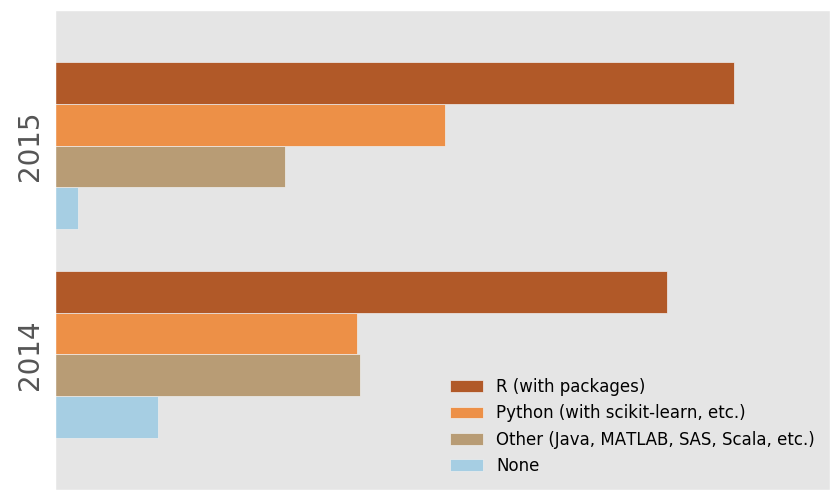
\includegraphics[width=15cm]{figuras/poll-lang}}
	}{
		\Fonte{KDNuggets 2015 poll: Primary programming language for Analytics, Data Mining, Data Science tasks}
	}	
\end{figure}

\subsection{Principais ferramentas}
\label{subsec:ferramentas}
Muitas vezes não é necessáro desenvolver um sitema machine learning para que se obtenha resultados satisfátórios, pois existem
ferramentas focadas em automatizar algumas tarefas para fazer \textbf{data-mining}, preparar os dados  ou visualiza-los de forma mais 
ilustrativa e simples. 

  






    